\section{Evaluating State-of-the-art RMs on \benchmark} \label{sec:evaluation}

\begin{figure*}[t!]
    \begin{subfigure}[t]{\textwidth}
        \centering
        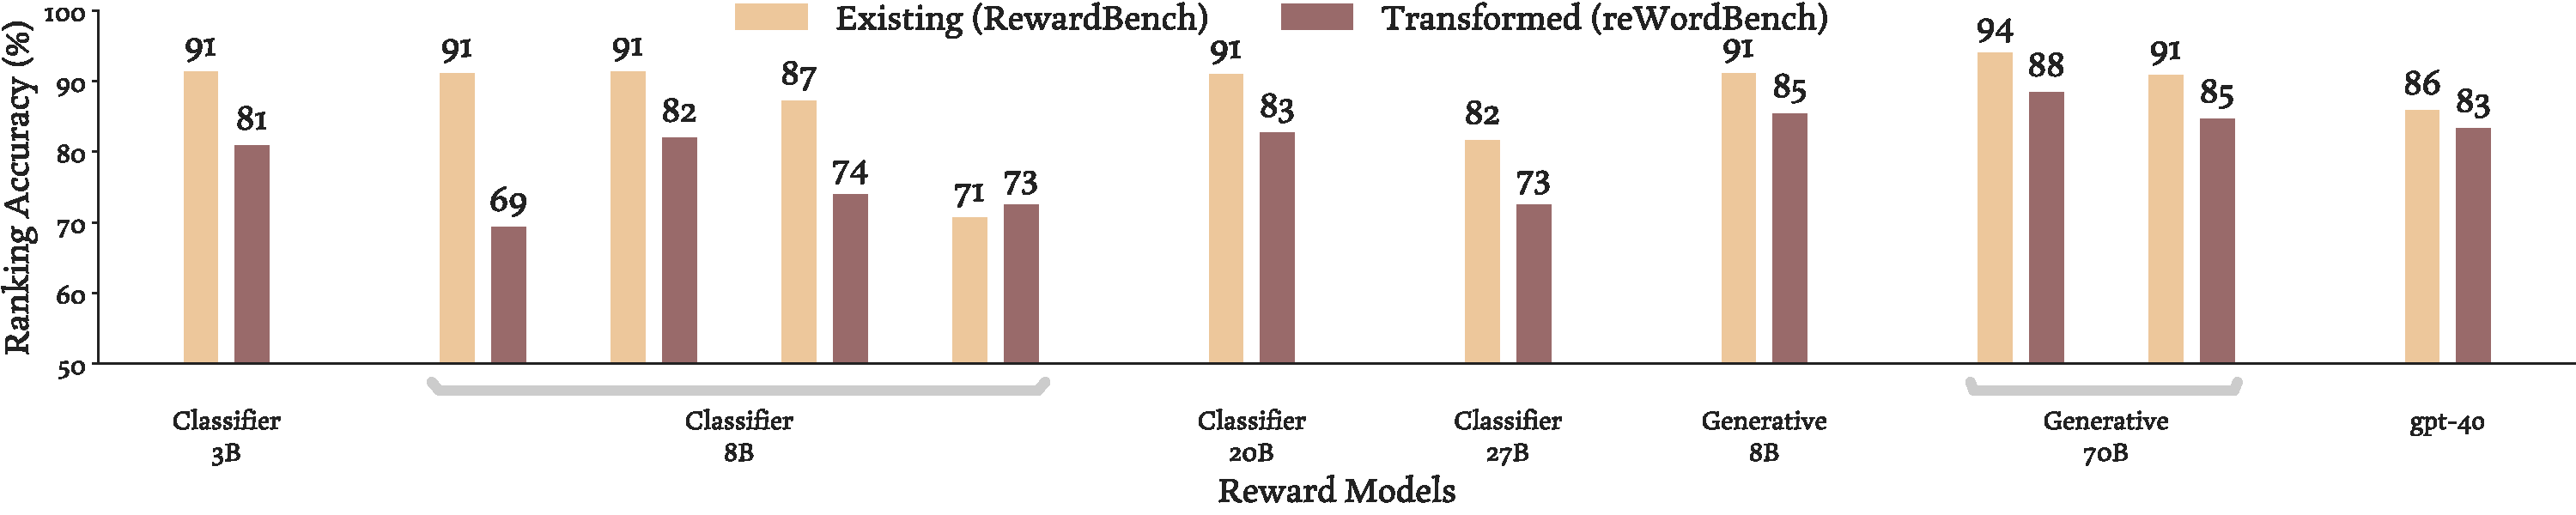
\includegraphics[width=\textwidth]{figures/consistency_rewardbench_pretrained_perturbations_avg_first_Controlled.pdf}
        \iflongversion
        \else
        \vspace{-6mm}
        \fi
        \caption{Controlled transformations. The specific model IDs are in \S\ref{sec:rm-selection}, in the same order.}
        \label{fig:pretrained-rms-controlled}
    \end{subfigure}
    \iflongversion
    \else
    \fi
    \begin{subfigure}[t]{\textwidth}
        \centering
        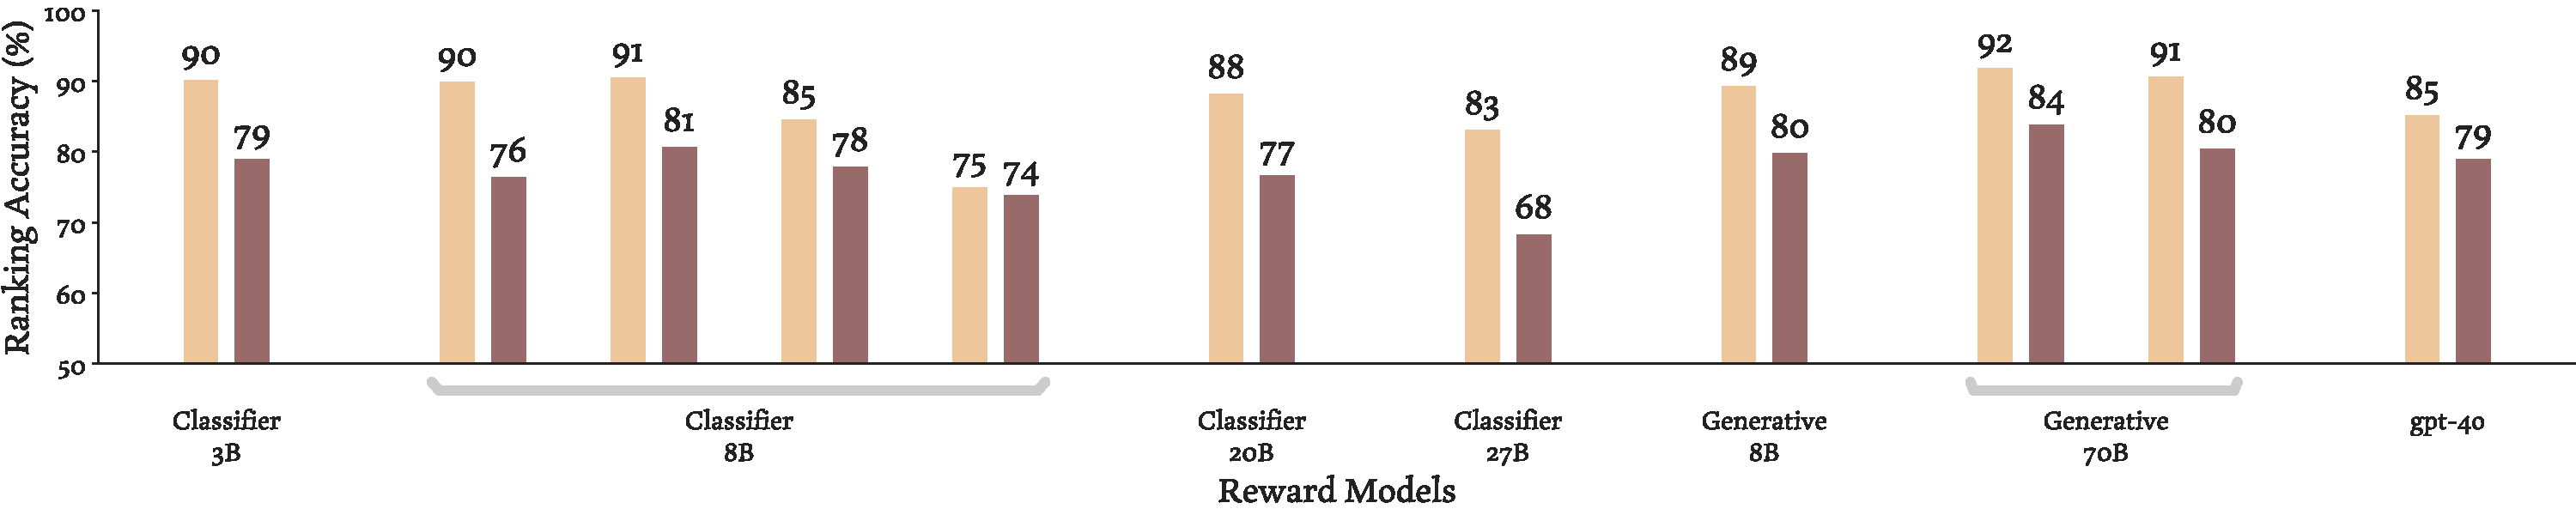
\includegraphics[width=\textwidth]{figures/consistency_rewardbench_pretrained_perturbations_avg_first_Natural.pdf}
        \iflongversion
        \else
        \vspace{-6mm}
        \fi
        \caption{Natural transformations. The specific model IDs are in \S\ref{sec:rm-selection}, in the same order.}
        \label{fig:pretrained-rms-natural}
    \end{subfigure}
    \iflongversion
    \else
    \fi
    \begin{subfigure}[t]{\textwidth}
        \centering
        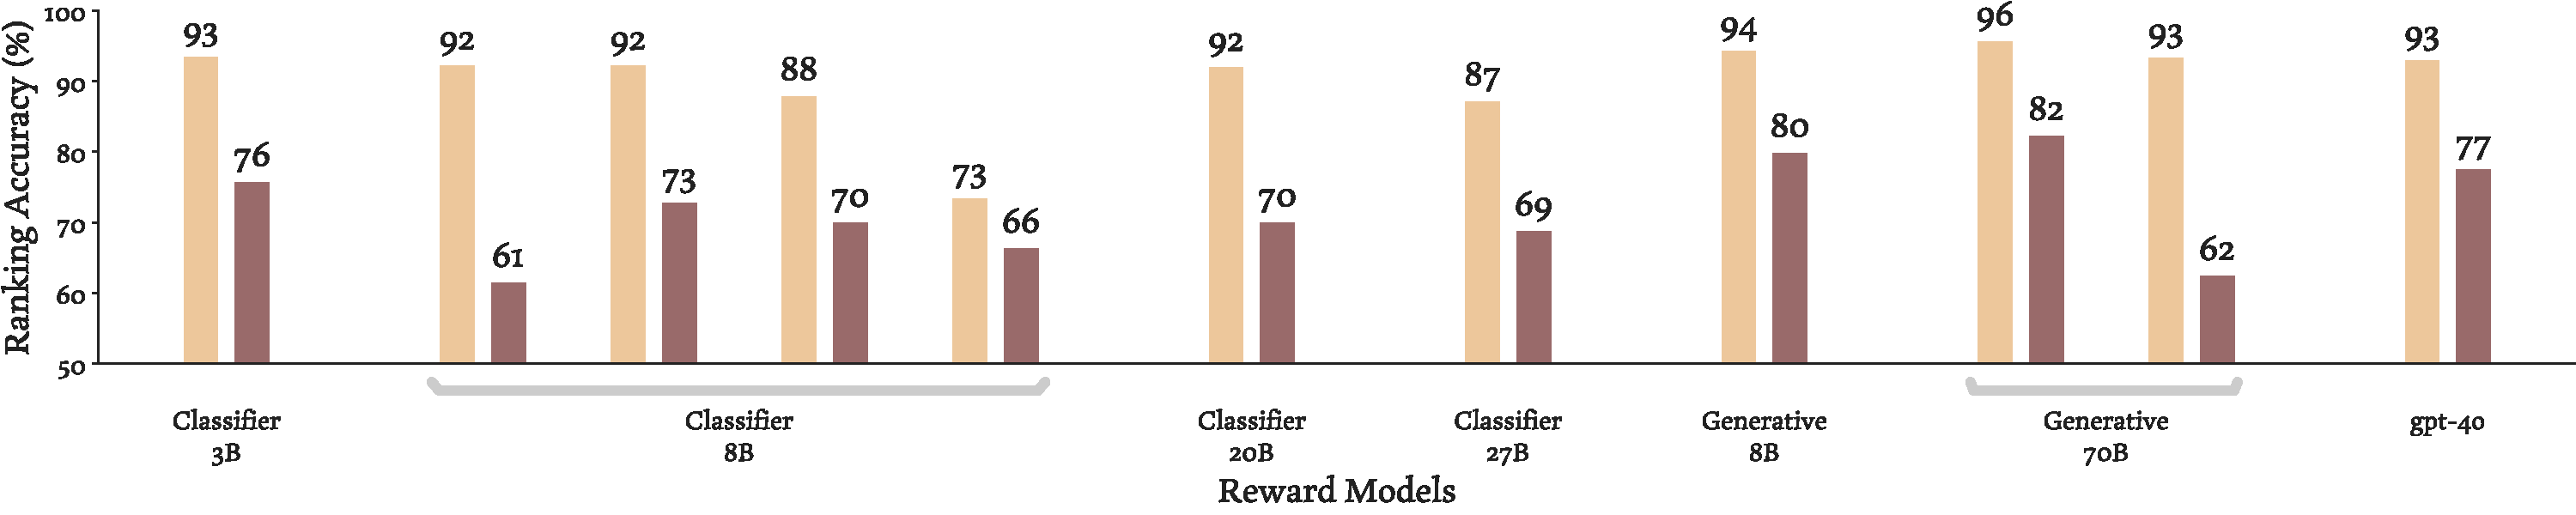
\includegraphics[width=\textwidth]{figures/consistency_rewardbench_pretrained_perturbations_avg_first_Targeted.pdf}
        \iflongversion
        \else
        \vspace{-6mm}
        \fi
        \caption{Domain-targeted transformations. The specific model IDs are in \S\ref{sec:rm-selection}, in the same order.}
        \label{fig:pretrained-rms-targeted}
    \end{subfigure}
    \iflongversion
    \else
    \vspace{-2mm}
    \fi
    \caption{
    \iflongversion
    The ranking accuracy of reward models
    \else
    RM ranking accuracy
    \fi
    under meaning- or ranking-preserving transformations. \textbf{SOTA RMs consistently
    \iflongversion
    suffer from performance degradation
    \else
    degrade in accuracy
    \fi
    when inputs are
    \iflongversion
    slightly
    \fi
    transformed.} Full results broken down by \iflongversion specific \else\fi transformations are in \S\ref{sec:full-results}.}
    \iflongversion
    \else
    \vspace{-4mm}
    \fi
    \label{fig:pretrained-rms}
\end{figure*}


We evaluate 7 top classifier RMs on RewardBench, one 3B-sized, four 8B-sized, and two 20-30B-sized.
We also consider 3 top generative LM-based RMs\iflongversion on RewardBench\else\fi, one 8B-sized and two 70B-sized, where the prompt and two responses are embedded in a template and the LM indicates a preferred response.
Furthermore, we evaluate GPT-4o~\citep{gpt4} as an RM.
To obtain RM preference, we compare the assigned scores to the responses for classifier RMs, and the next token probability for symbol tokens that represent the two responses (\texttt{A} and \texttt{B}) for generative \iflongversion RMs (see the individual model webpages in \S\ref{sec:rm-selection} for details). \else RMs.\fi For GPT-4o, we use prompting~(\S\ref{sec:instructions}).
See \S\ref{sec:rm-selection} for our selection criteria and the RMs selected.



Figure~\ref{fig:pretrained-rms} shows the ranking accuracy
\iflongversion
drop of RMs,
\else
drop,
\fi
broken down by the 3 \benchmark categories.
\S\ref{sec:full-results} shows more fine-grained results.
\textbf{We see substantial
\iflongversion
accuracy
\fi
degradation across transformations and models}. While the degradations are usually larger for more adversarial transformations, in many cases deteriorating to below-random accuracy, we also see large drops with the natural transformations.

We make some further observations.
First, \textbf{this brittleness is shared across model types and sizes}---both classifier and generative RMs, and both smaller and larger models, suffer from similar drops.
Second, \textbf{different models differ in robustness properties}. 
In fact, the best classifier RM on the original RewardBench (out of the 7 we consider) is no longer the best after 18/28 of our transformations.
This means that the relative ranking between models changes under transformations; therefore, not only does RewardBench performance overestimate RM capability, but it does not necessarily faithfully reflect the RM quality \emph{ranking} either (if \benchmark better measures RM quality).
Third, \textbf{while some transformations do not lead to substantial accuracy drops, they still drastically change the predicted rewards} (see \S\ref{sec:score-changes}), which may cause instability in RL-based alignment; thus, Figure~\ref{fig:pretrained-rms} can be considered a ``lower bound'' on the impact of RM brittleness.
